\section{Architecture and Training}

\subsection{Corruption Rate}

\begin{table}[t]
\begin{tabular}{ | m{2cm} | m{1cm} | m{1cm} | m{1cm} | m{1cm} | m{1cm} | m{1cm} | }
  \hline
  & NC & MB & MS & VAR & RET & SL \\
  \hline
  \hline
  100\% & 60.0 & 48.2 & 64.0 & \textbf{37.3} & 54.3 & 26.7 \\
  \hline
  75\% & \textbf{70.4} & \textbf{51.3} & \textbf{71.8} & 34.4 & \textbf{55.1} & \textbf{42.6} \\
  \hline
  50\% & 62.0 & 43.7 & 61.2 & 25.0 & 47.4 & 26.1 \\
  \hline
  25\% & 67.9 & 41.6 & 65.6 & 19.6 & 50.3 & 33.3 \\
  \hline
\end{tabular}
\caption{Results}
\label{corruption_rate_table}
\end{table}

Because the source sequence and target sequence are almost the same and the errors are self-introduced, it is fair to ask what the optimal corruption rate for the input is. To test this the model was trained with four different corruption rates, 100\%, 75\%, 50\% and 25\%. The results can be seen in table \ref{corruption_rate_table}.

For almost all corruptions the model trained with a corruption rate of 75\% posts the best result. The models with lower percentages don't pick up on the errors as well while the model with the 100\% corruption rate lacks the ground truth. In general the model learns to correct all of the introduced errors. It performs especially well when inputting a sequence missing a single semicolon which is of course also the simplest task to solve. However the model is also able to correct the other errors reasonably well. A missing bracket or an incorrect return type are corrected most of the time while the model has a little more trouble correcting a misspelled variable or realigning switched lines. A more detailed analysis for the different error types is given in section \ref{error_analysis}.

What's also interesting to see is how well the model performs on uncorrupted sequences. Even the model with 100\% corruption rate, i.e. which never gets an uncorrupted sequence as input, manages to not introduce any new errors into an uncorrupted sequence most of the time. This indicates that the model obtains some understanding of the input and only corrects where necessary.

\subsection{Attention Mechanism}

\begin{figure}[p]
\centering
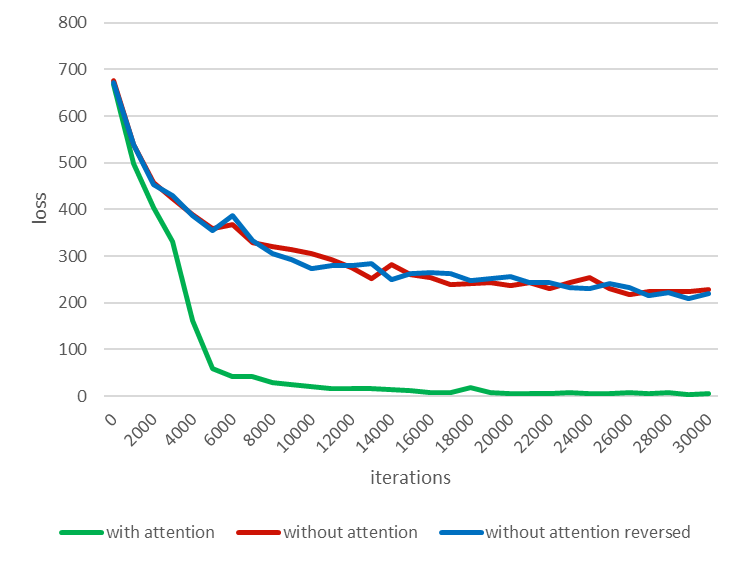
\includegraphics[width=0.9\linewidth]{attention_chart}
\caption{Line chart showing the loss of different models over time.}
\label{attention_chart}
\end{figure}

Of course it can also be asked if the attention mechanism is necessary for the model, after all it increases complexity and training duration. To test this, the model was constructed without an attention mechanism on top of the decoder. This model was then trained twice, once with the same input the regular model got and once with the input reversed. The reversion of the input is a technique proposed in \cite{seq2seq}, the idea being to introduce more short term dependencies while the average distance of the dependencies stays the same. This is not necessary for the regular model because the attention mechanism allows the model to take a peek of the encoder state at any given timestep.

The experiments revealed the attention mechanism to be an essential part of the model because the models without the mechanism weren't able to solve the given task. These models never learnt to repeat the input sequence probably because they couldn't pass all information from the encoder to the decoder in a single vector.

For the first couple of thousand iterations all models learnt roughly the same things, namely the general structure of the desired output. The models would start to begin the output sequence with \texttt{public ...(...)\{} and end and it with \texttt{\}<eos>}. In between they added mostly passages they remembered from training. However after about 4,000 iterations the model with the attention mechanism learnt to utilise the mechanism to its full potential and started repeating the input sequence. This resulted in rapid performance improvement. The loss of the different configurations as a function over iterations can be seen in figure \ref{attention_chart}.

The reversion of the input sequence helped the model to learn a little bit faster and perform a little bit better but overall it made almost no difference. The model was still not able to solve the task.

\subsection{RNN type}

\begin{figure}[p]
\centering
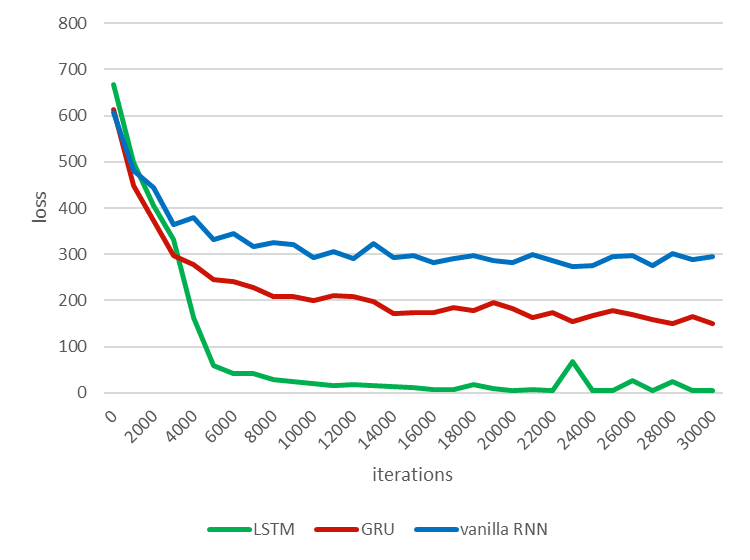
\includegraphics[width=0.9\linewidth]{cell_type_chart}
\caption{Line chart showing the loss of different models over time.}
\label{cell_type_chart}
\end{figure}

In subsection \ref{rnn_types} three types of RNNs were listed: vanilla RNNs, LSTMs and GRUs. In this experiment, for each type a model is trained with the respective RNN type.

\section{Error analysis}
\label{error_analysis}

\subsection{Uncorrupted}

similar characters. *(42), +(43)

incorrect switching of lines

tolerance: 79.6\%

wrong switch: 4.8\%

\subsection{Brackets}

balanced brackets: 77.2\%

matching brackets: 76.9\%

\subsection{Semicolon}

tolerance: 81.7\%

wrong switch: 3.2\%

correct number of semicolons: 97.0\%

\subsection{Variable}

\begin{figure}[p]
\centering
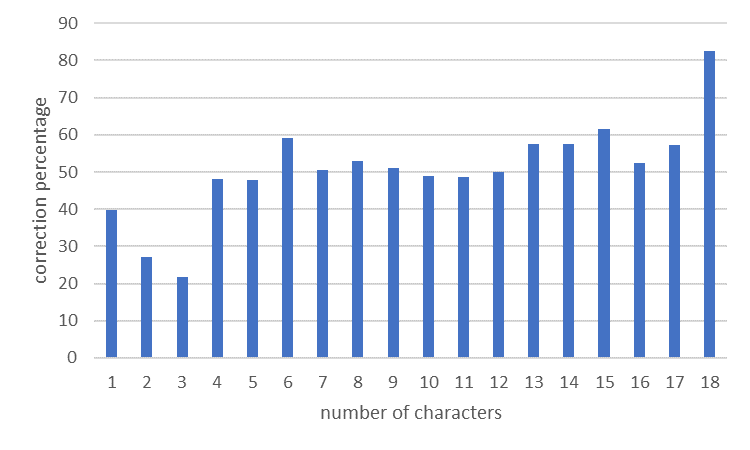
\includegraphics[width=0.9\linewidth]{variables_chart}
\caption{Correction percentage for variables evaluated for different lengths. Only lengths with more than 10 examples were considered.}
\label{variables_chart}
\end{figure}

Including corrected wrong instance: 45.6\%

\subsection{Return type}

different percentages

\subsection{Switch}

\begin{table}[h]
\begin{tabular}{ | m{1cm} | m{1cm} | m{1cm} | m{1cm} | }
  \hline
  \(\leftrightarrow\) & VD & MI & AS \\
  \hline
  \hline
  VD & - & 53.3 & \textbf{59.3} \\
  \hline
  MI & 0.0 & - & 13.0 \\
  \hline
  AS & 0.0 & 9.8 & - \\
  \hline
\end{tabular}
\caption{VC = Variable Declaration, MI = method invocation, AS = assignment.}
\label{switch_table}
\end{table}
